\documentclass[a4paper,11pt]{article}
\usepackage[slovene]{babel}
\usepackage[utf8]{inputenc}
\usepackage[T1]{fontenc}
\usepackage{amsmath}
\usepackage{graphicx}
\usepackage{booktabs}
\usepackage{url}
\usepackage{placeins}
\usepackage{tikz}
\usetikzlibrary{patterns}
\usepackage{algorithm}
\usepackage[noend]{algpseudocode}
\floatname{algorithm}{Algoritem}
\algrenewcommand\algorithmicfor{\textbf{za}}
\algrenewcommand\algorithmicdo{\textbf{naredi}}
\algrenewcommand\algorithmicif{\textbf{če}}
\algrenewcommand\algorithmicthen{\textbf{potem}}
\algrenewcommand\algorithmicrequire{\textbf{Vhod:}}
\algrenewcommand\algorithmicensure{\textbf{Izhod:}}

\title{Reševanje 2D enačbe prenosa toplote z metodo končnih diferenc}
\author{Aljaž Brodar}
\date{\today}

\begin{document}
	
	\maketitle
	\newpage
	\tableofcontents
	\newpage
	
	\section{Matematični model}
	
	V projektu rešujemo dvodimenzionalno enačbo prenosa toplote
	\begin{equation}
		\frac{\partial T}{\partial t} = D \nabla^2 T
		\label{eq:toplota}
	\end{equation}
	z metodo končnih diferenc. Enačba opisuje temperaturno porazdelitev objekta in kako se ta spreminja s časom.
	
	\subsection{Enačba v eni dimenziji}
	
	Izpeljava v tem razdelku sledi \cite{dawkins}. Najprej definiramo osnovne pojme za enodimenzionalno različico problema:
	\begin{align*}
		T(x, t)       &= \text{temperatura v točki } x \text{ ob času } t, \\
		c(x)          &= \text{specifična toplota}, \\
		\rho(x)       &= \text{gostota}, \\
		\varphi(x, t) &= \text{gostota toplotnega toka}, \\
		Q(x, t)       &= \text{toplotni izvor na enoto prostornine in časa}.
	\end{align*}
	
	Specifična toplota materiala, $c(x) > 0$, je količina toplote, ki jo potrebujemo, da enoti mase materiala dvignemo temperaturo za eno enoto.
	
	Gostota predstavlja maso na enoto volumna materiala.
	
	Gostota toplotnega toka je fizikalna količina, ki pove, koliko toplote na enoto površine preteče v časovni enoti.
	
	Toplotni izvor na enoto prostornine in časa predstavlja notranje vire toplote. Če je $Q(x, t) > 0$, se sistemu v točki $x$ ob času $t$ dovaja toplota. V nasprotnem primeru, $Q(x, t) < 0$, se toplota sistemu odvaja.
	
	S temi količinami je enačba prenosa toplote
	\begin{equation}
		c(x)\rho(x) \frac{\partial T}{\partial t} = -\frac{\partial \varphi}{\partial x} + Q(x, t).
		\label{eq:bilanca1d}
	\end{equation}
	
	S pomočjo Fourierovega zakona lahko gostoto toplotnega toka odstranimo iz enačbe. Zakon zapišemo kot
	\begin{equation}
		\varphi(x, t) = -K_0(x) \frac{\partial T}{\partial x},
		\label{eq:fourier1d}
	\end{equation}
	kjer je $K_0 > 0$ toplotna prevodnost materiala in meri njegovo sposobnost prevajanja toplote. Bolje kot material prevaja toploto, večja je količina $K_0(x)$.
	
	Poglejmo, kako zakon modelira prenos toplote. Če je temperatura na območju konstantna, $\frac{\partial T}{\partial x} = 0$, potem ni prenosa toplote. Če je na območju temperaturna razlika, potem toplota preide iz toplejšega dela k hladnejšemu delu. Torej, če je topleje na desni strani, toplota teče proti levi. V tem primeru velja $\frac{\partial T}{\partial x} > 0$ (tj.\ temperatura se poveča, ko se premaknemo desno) in posledično dobimo $\varphi < 0$. Podobno velja v nasprotnem primeru, ko je toplejši del na levi strani: $\frac{\partial T}{\partial x} < 0$, iz česar sledi $\varphi > 0$, kjer toplota potuje v desno stran. Opazimo, da večja kot je temperaturna razlika oz.\ količina $\frac{\partial T}{\partial x}$, večji je prenos toplote.
	
	Če vstavimo Fourierov zakon v enačbo prenosa toplote, dobimo
	\begin{equation}
		c(x)\rho(x) \frac{\partial T}{\partial t} = \frac{\partial}{\partial x}\left(K_0(x) \frac{\partial T}{\partial x}\right) + Q(x, t).
	\end{equation}
	Predpostavimo, da so naslednje količine konstante: $c(x) = c$, $\rho(x) = \rho$ in $K_0(x) = K_0$. V primeru enodimenzionalne palice bi rekli, da je njen material homogen. Pod to predpostavko postane enačba prenosa toplote
	\begin{equation}
		c\rho \frac{\partial T}{\partial t} = K_0 \frac{\partial^2 T}{\partial x^2} + Q(x, t).
		\label{eq:eq3}
	\end{equation}
	Enačbo delimo s produktom $c\rho$ in definiramo toplotno difuzivnost kot $D = \frac{K_0}{c\rho}$. Toplotna enačba je potem
	\begin{equation}
		\frac{\partial T}{\partial t} = D \frac{\partial^2 T}{\partial x^2} + \frac{Q(x, t)}{c\rho}.
		\label{eq:eq4}
	\end{equation}
	V primeru, ko nimamo notranjih virov, nastavimo $Q(x, t) = 0$.
	
	\subsection{Robni pogoji}
	
	Sedaj, ko smo zapisali toplotno enačbo v eni dimenziji, opišemo dve vrsti robnih pogojev, ki ju bomo kasneje uporabili pri reševanju problema. To so Dirichletovi in Neumannovi robni pogoji. Robni pogoji opišejo temperaturo in prenos toplote na mejah domene (na primer v eni dimenziji govorimo o mejah palice). Dirichletov pogoj je tisti, kjer na meji nastavimo predpisano vrednost spremenljivke, medtem ko je Neumannov pogoj tisti, ki določa vrednost odvoda rešitve na meji.
	
	\subsection{Enačba v dveh dimenzijah}
	
	Preden zapišemo enačbo v dveh dimenzijah, predstavimo novo matematično notacijo.
	
	Operator $\nabla$ je definiran kot
	\begin{equation}
		\nabla = \frac{\partial}{\partial x}\vec{i} + \frac{\partial}{\partial y}\vec{j}.
	\end{equation}
	Lahko si ga predstavljamo kot funkcijo, ki prejme funkcije kot argumente (namesto števil, ki so običajno argumenti). Funkcija, ki jo vstavimo v operator, se pretvori v parcialne odvode:
	\begin{equation}
		\nabla f = \frac{\partial f}{\partial x}\vec{i} + \frac{\partial f}{\partial y}\vec{j}.
	\end{equation}
	
	Omenjeni operator nam omogoča tudi zapis divergence funkcije:
	\begin{equation}
		\nabla \cdot f = \frac{\partial f}{\partial x} + \frac{\partial f}{\partial y}.
	\end{equation}
	
	Kasneje se pojavi tudi
	\begin{equation}
		\nabla \cdot (\nabla f)
		= \frac{\partial}{\partial x}\left(\frac{\partial f}{\partial x}\right)
		+ \frac{\partial}{\partial y}\left(\frac{\partial f}{\partial y}\right)
		= \frac{\partial^2 f}{\partial x^2} + \frac{\partial^2 f}{\partial y^2},
	\end{equation}
	kar zapišemo tudi kot
	\begin{equation}
		\nabla^2 f = \frac{\partial^2 f}{\partial x^2} + \frac{\partial^2 f}{\partial y^2}.
	\end{equation}
	Operator $\nabla^2$ je znan tudi kot Laplaceov operator.
	
	Enačbo prenosa toplote v dveh dimenzijah zapišemo kot
	\begin{equation}
		c\rho \frac{\partial T}{\partial t} = -\nabla \cdot \varphi + Q(x, y, t).
	\end{equation}
	
	Fourierov zakon v več dimenzijah je enak
	\begin{equation}
		\varphi = -K_0 \nabla T.
	\end{equation}
	
	Ponovno upoštevamo zakon v enačbi prenosa toplote:
	\begin{equation}
		c\rho \frac{\partial T}{\partial t} = \nabla \cdot (K_0 \nabla T) + Q.
	\end{equation}
	
	V primeru, da so $c$, $\rho$ in $K_0$ konstante, velja
	\begin{equation}
		\frac{\partial T}{\partial t} = D \nabla^2 T + \frac{Q}{c\rho}.
	\end{equation}
	V obravnavanem primeru ni notranjih toplotnih virov, $Q = 0$, zato dobimo enačbo
	\begin{equation}
		\frac{\partial T}{\partial t} = D \nabla^2 T.
	\end{equation}
	
	\subsection{Domena}
	Pri reševanju problema obravnavamo pravokotno domeno: $0 \leq x \leq L$ in $0 \leq y \leq H$ (Slika~\ref{fig:domena}).
	V obeh kasneje opisanih testnih primerih velja $L = H = 1$ ter $T(x, y, t = 0) = 50$.
	
	\begin{figure}[htbp]
		\centering
		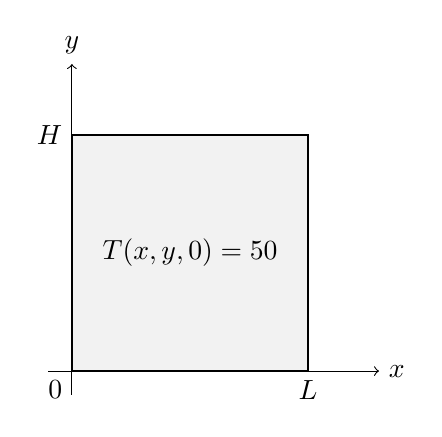
\begin{tikzpicture}[scale=3]
			% osi x in y
			\draw[->] (-0.1, 0) -- (1.3, 0) node[right] {$x$};
			\draw[->] (0, -0.1) -- (0, 1.3) node[above] {$y$};
			% domena
			\draw[thick, fill=gray!10] (0, 0) rectangle (1, 1);
			% oznake na oseh
			\node[below left] at (0, 0) {$0$};
			\node[below] at (1, 0) {$L$};
			\node[left] at (0, 1) {$H$};
			% notranjost
			\node at (0.5, 0.5) {$T(x, y, 0) = 50$};
		\end{tikzpicture}
		\caption{Pravokotna domena problema.}
		\label{fig:domena}
	\end{figure}
	
	\subsection{Testna primera}
	
	V prvem testnem primeru veljajo naslednji robni pogoji:
	\begin{align*}
		&\text{levi rob:}    && T(0, y) = 100, \\
		&\text{desni rob:}   && T(L, y) = 0, \\
		&\text{spodnji rob:} && \frac{\partial T}{\partial y}(x, 0) = 0, \\
		&\text{zgornji rob:} && \frac{\partial T}{\partial y}(x, H) = 0.
	\end{align*}
	Analitična stacionarna rešitev je
	\begin{equation}
		T(x) = 100 \left(1 - \frac{x}{L}\right).
		\label{eq:resitev1}
	\end{equation}
	Robni pogoji so prikazani na sliki~\ref{fig:primer1}.
	
	\begin{figure}[h]
		\centering
		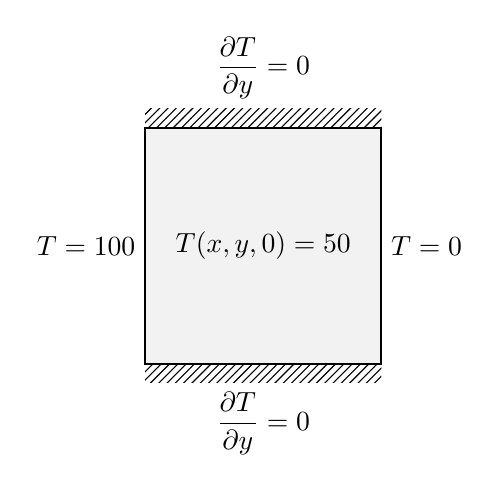
\begin{tikzpicture}[scale=3]
			% izolacija (srafura) zgoraj in spodaj
			\fill[pattern=north east lines] (0, 1) rectangle (1, 1.08);
			\fill[pattern=north east lines] (0, -0.08) rectangle (1, 0);
			% domena
			\draw[thick, fill=gray!10] (0, 0) rectangle (1, 1);
			% oznake robov
			\node[left]  at (0, 0.5) {$T = 100$};
			\node[right] at (1, 0.5) {$T = 0$};
			\node[above] at (0.5, 1.08) {$\dfrac{\partial T}{\partial y} = 0$};
			\node[below] at (0.5, -0.08) {$\dfrac{\partial T}{\partial y} = 0$};
			% notranjost
			\node at (0.5, 0.5) {$T(x, y, 0) = 50$};
		\end{tikzpicture}
		\caption{Robni pogoji prvega testnega primera. Črtkan vzorec označuje izoliran rob.}
		\label{fig:primer1}
	\end{figure}
	
	V drugem testnem primeru veljajo naslednji robni pogoji:
	\begin{align*}
		&\text{levi rob:}    && T(0, y) = 0, \\
		&\text{desni rob:}   && T(1, y) = 0, \\
		&\text{spodnji rob:} && T(x, 0) = 100 \sin(\pi x), \\
		&\text{zgornji rob:} && \frac{\partial T}{\partial y}(x, 1) = 0.
	\end{align*}
	Analitična rešitev je
	\begin{equation}
		T(x, y) = 100\,\frac{\cosh[\pi(1 - y)]}{\cosh \pi}\,\sin(\pi x).
		\label{eq:resitev2}
	\end{equation}
	Robni pogoji so prikazani na sliki~\ref{fig:primer2}.
	
	\begin{figure}[h]
		\centering
		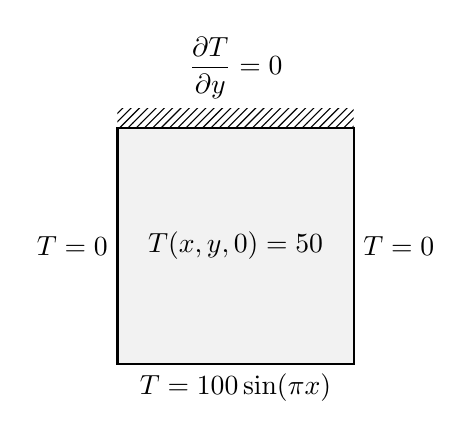
\begin{tikzpicture}[scale=3]
			% izolacija (srafura) zgoraj
			\fill[pattern=north east lines] (0, 1) rectangle (1, 1.08);
			% domena
			\draw[thick, fill=gray!10] (0, 0) rectangle (1, 1);
			% oznake robov
			\node[left]  at (0, 0.5) {$T = 0$};
			\node[right] at (1, 0.5) {$T = 0$};
			\node[above] at (0.5, 1.08) {$\dfrac{\partial T}{\partial y} = 0$};
			\node[below] at (0.5, 0) {$T = 100 \sin(\pi x)$};
			% notranjost
			\node at (0.5, 0.5) {$T(x, y, 0) = 50$};
		\end{tikzpicture}
		\caption{Robni pogoji drugega testnega primera. Črtkan vzorec označuje izoliran rob.}
		\label{fig:primer2}
	\end{figure}
	
	\subsection{Ustaljeno stanje}
	
	Na začetku ima plošča povsod temperaturo $50$, robni pogoji pa jo začnejo spreminjati. Temperatura se sprva spreminja hitro, nato vse počasneje, dokler se ne ustali. Takrat je vsaka točka dosegla svojo končno vrednost; temu rečemo ustaljeno (stacionarno) stanje.
	
	V ustaljenem stanju se temperatura s časom ne spreminja več, torej velja $\frac{\partial T}{\partial t} = 0$. Če to vstavimo v enačbo~\eqref{eq:toplota}, dobimo
	\begin{equation}
		\nabla^2 T = 0,
		\label{eq:laplace}
	\end{equation}
	kar imenujemo Laplaceova enačba. Ker smo enačbo lahko delili z $D$, ustaljeno stanje od $D$ ni odvisno: $D$ vpliva le na to, kako hitro plošča ustaljeno stanje doseže.
	
	\newpage
	\section{Numerična metoda}
	
	Najprej zgradimo dvodimenzionalno mrežo diskretnih točk, na kateri računamo rešitev.
	
	% =====================================================================
	\subsection{Mreža}
	
	Uporabimo dvodimenzionalno kartezično mrežo, ki jo sestavljata dve družini mrežnih črt, vzporednih s koordinatnima osema. Dve črti iz različnih družin se sekata v natanko enem vozlišču mreže; takšni mreži rečemo strukturirana mreža. V smeri $x$ diskretizacija uporablja črte $i = 0, \dots, N_x$, v smeri $y$ pa črte $j = 0, \dots, N_y$. Vsako vozlišče mreže ima tako dve prostorski koordinati, zato potrebujemo dva indeksa: po enega za vsako od črt, ki se v vozlišču sekata. Temperaturo v srednjem vozlišču na sliki~\ref{fig:mreza} na primer označimo s $T_{i,j}$.
	
	\begin{figure}[htbp]
		\centering
		\begin{tikzpicture}[scale=1.6]
			% osi
			\draw[->] (0, 0) -- (4.2, 0) node[right] {$x$};
			\draw[->] (0, 0) -- (0, 4.2) node[above] {$y$};
			% mrezne crte (crtkane)
			\foreach \k in {1, 2, 3} {
				\draw[gray!50, dashed] (\k, 0.3) -- (\k, 3.7);
				\draw[gray!50, dashed] (0.3, \k) -- (3.7, \k);
			}
			% oznake indeksov na oseh
			\foreach \k/\lab in {1/{i-1}, 2/{i}, 3/{i+1}} {
				\draw (\k, 0.08) -- (\k, -0.08) node[below] {$\lab$};
			}
			\foreach \k/\lab in {1/{j-1}, 2/{j}, 3/{j+1}} {
				\draw (0.08, \k) -- (-0.08, \k) node[left] {$\lab$};
			}
			% vozlisca z oznakami
			\foreach \a/\la in {1/{i-1}, 2/{i}, 3/{i+1}} {
				\foreach \b/\lb in {1/{j-1}, 2/{j}, 3/{j+1}} {
					\fill (\a, \b) circle (0.06);
					\node[above, font=\footnotesize] at (\a, \b) {$T_{\la,\lb}$};
				}
			}
		\end{tikzpicture}
		\caption{Del dvodimenzionalne kartezične mreže: vozlišče $(i, j)$ in njegovi sosedje.}
		\label{fig:mreza}
	\end{figure}
	
	% =====================================================================
	\subsection{Diskretizacija enačbe modela}
	
	Izpeljava v tem razdelku sledi \cite{mooc}. Začnemo z diskretizacijo v eni dimenziji in jo kasneje razširimo v dve.
	
	\subsubsection{Končne diference za prvi odvod}
	
	Iz definicije odvoda (in z odstranitvijo limite) vemo, da za dovolj majhen $\Delta x$ velja
	\begin{equation}
		\frac{\partial T}{\partial x} \approx \frac{T(x + \Delta x) - T(x)}{\Delta x}.
	\end{equation}
	Navedeno formulo lahko uporabimo v poljubni točki $x_i$. Navedena formula pa ni edini način aproksimacije odvoda. Geometrijska interpretacija prvega odvoda $\frac{\partial T}{\partial x}$ v izbrani točki predstavlja smerni koeficient tangente na krivuljo $T(x)$. Na sliki~\ref{fig:diference} je tangenta v točki $x_i$ označena kot točen odvod. Če formulo uporabimo v točki $x_i$, odvod aproksimiramo s pomočjo naslednje točke mreže; takrat jo imenujemo prema diferenca (angl.\ \emph{forward difference}). Kot kaže slika, lahko prostorski odvod ocenimo tudi s pomočjo točke pred $x_i$; v tem primeru govorimo o obratni diferenci. Uporabimo lahko tudi točki na obeh straneh $x_i$ in dobimo centralno diferenco, pri kateri je v imenovalcu $2\Delta x$.
	
	\begin{figure}[htbp]
		\centering
		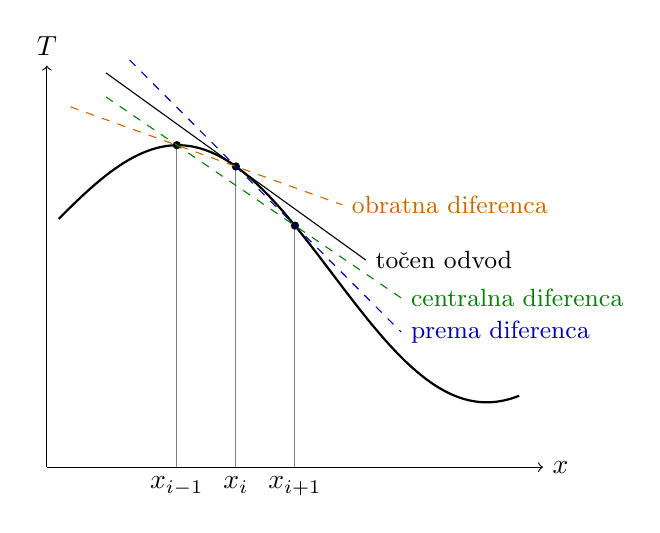
\begin{tikzpicture}[scale=1.5,
			declare function={
				f(\x) = 2 + 0.9*sin(deg(1.3*\x)) - 0.15*\x;
				fp(\x) = 0.9*1.3*cos(deg(1.3*\x)) - 0.15;
			}]
			\def\xc{1.6}
			\def\h{0.5}
			\pgfmathsetmacro{\xa}{\xc-\h}
			\pgfmathsetmacro{\xb}{\xc+\h}
			\pgfmathsetmacro{\fa}{f(\xa)}
			\pgfmathsetmacro{\fc}{f(\xc)}
			\pgfmathsetmacro{\fb}{f(\xb)}
			\pgfmathsetmacro{\sex}{fp(\xc)}
			\pgfmathsetmacro{\sfw}{(\fb-\fc)/\h}
			\pgfmathsetmacro{\sbw}{(\fc-\fa)/\h}
			\pgfmathsetmacro{\sce}{(\fb-\fa)/(2*\h)}
			% osi
			\draw[->] (0, 0) -- (4.2, 0) node[right] {$x$};
			\draw[->] (0, 0) -- (0, 3.4) node[above] {$T$};
			% krivulja
			\draw[thick, domain=0.1:4, samples=100] plot (\x, {f(\x)});
			% navpicne crte in oznake
			\foreach \p/\lab in {\xa/{x_{i-1}}, \xc/{x_i}, \xb/{x_{i+1}}} {
				\draw[gray] (\p, 0) -- (\p, {f(\p)});
				\fill ({\p}, {f(\p)}) circle (0.035);
				\node[below] at (\p, 0) {$\lab$};
			}
			% premice
			\draw[black]                   ({\xc-1.1}, {\fc-1.1*\sex}) -- ({\xc+1.1}, {\fc+1.1*\sex})
			node[right, font=\small] {točen odvod};
			\draw[blue!70!black, dashed]   ({\xc-0.9}, {\fc-0.9*\sfw}) -- ({\xc+1.4}, {\fc+1.4*\sfw})
			node[right, font=\small] {prema diferenca};
			\draw[orange!80!black, dashed] ({\xc-1.4}, {\fc-1.4*\sbw}) -- ({\xc+0.9}, {\fc+0.9*\sbw})
			node[right, font=\small] {obratna diferenca};
			\draw[green!50!black, dashed]  ({\xa-0.6}, {\fa-0.6*\sce}) -- ({\xb+0.9}, {\fb+0.9*\sce})
			node[right, font=\small] {centralna diferenca};
		\end{tikzpicture}
		\caption{Tri končne diference za oceno prvega odvoda v točki $x_i$.}
		\label{fig:diference}
	\end{figure}
	
	Torej poznamo tri različne vrste aproksimacij s končnimi diferencami:
	\begin{enumerate}
		\item prema diferenca: uporabi $x_i$ in $x_i + \Delta x$;
		\item obratna diferenca: uporabi $x_i$ in $x_i - \Delta x$;
		\item centralna diferenca: uporabi sosednji točki $x_i - \Delta x$ in $x_i + \Delta x$.
	\end{enumerate}
	S formulami zapišemo:
	\begin{align}
		\frac{\partial T}{\partial x} &\approx \frac{T(x_{i+1}) - T(x_i)}{\Delta x}       && \text{(prema)},     \\
		\frac{\partial T}{\partial x} &\approx \frac{T(x_i) - T(x_{i-1})}{\Delta x}       && \text{(obratna)},   \\
		\frac{\partial T}{\partial x} &\approx \frac{T(x_{i+1}) - T(x_{i-1})}{2\Delta x}  && \text{(centralna)}.
	\end{align}
	
	\subsubsection{Časovni odvod}
	
	Časovni odvod aproksimiramo s premo diferenco, kar ustreza eksplicitni Eulerjevi metodi:
	\begin{equation}
		\frac{\partial T}{\partial t} \approx \frac{T^{n+1}_{i,j} - T^{n}_{i,j}}{\Delta t}.
	\end{equation}
	
	\subsubsection{Drugi odvod}
	
	V enačbi prenosa toplote~\eqref{eq:toplota} opazimo prisotnost odvoda drugega reda. Tega geometrijsko predstavimo kot smerni koeficient tangente na krivuljo prvega odvoda. Drugi odvod v nadaljevanju diskretiziramo z metodo centralnih diferenc. Obravnavamo Taylorjevi vrsti za $T_{i+1}$ in $T_{i-1}$ okrog $x_i$:
	\begin{align}
		T_{i+1} &= T_i + \Delta x \frac{\partial T}{\partial x}\Big|_i + \frac{\Delta x^2}{2!} \frac{\partial^2 T}{\partial x^2}\Big|_i + \frac{\Delta x^3}{3!} \frac{\partial^3 T}{\partial x^3}\Big|_i + \mathcal{O}(\Delta x^4), \\
		T_{i-1} &= T_i - \Delta x \frac{\partial T}{\partial x}\Big|_i + \frac{\Delta x^2}{2!} \frac{\partial^2 T}{\partial x^2}\Big|_i - \frac{\Delta x^3}{3!} \frac{\partial^3 T}{\partial x^3}\Big|_i + \mathcal{O}(\Delta x^4),
	\end{align}
	pri čemer smo vse člene reda $\mathcal{O}(\Delta x^4)$ in višje zanemarili; gre za izredno majhne količine. Ko enačbi seštejemo, se členi z odvodi lihega reda pokrajšajo:
	\begin{equation}
		T_{i+1} + T_{i-1} = 2T_i + \Delta x^2 \frac{\partial^2 T}{\partial x^2}\Big|_i + \mathcal{O}(\Delta x^4).
	\end{equation}
	Rešimo za drugi odvod:
	\begin{equation}
		\frac{\partial^2 T}{\partial x^2}\Big|_i = \frac{T_{i+1} - 2T_i + T_{i-1}}{\Delta x^2} + \mathcal{O}(\Delta x^2).
		\label{eq:drugi_odvod}
	\end{equation}
	Centralna diferenca za drugi odvod je drugega reda natančnosti oz.\ ima napako reda $\mathcal{O}(\Delta x^2)$.
	
	\subsubsection{Eksplicitna shema v eni dimenziji}
	
	Sedaj lahko zapišemo diskretno različico enačbe toplote v eni dimenziji kot
	\begin{equation}
		\frac{T^{n+1}_i - T^n_i}{\Delta t} = D\,\frac{T^n_{i+1} - 2T^n_i + T^n_{i-1}}{\Delta x^2}.
	\end{equation}
	Rešimo za edino neznanko $T^{n+1}_i$:
	\begin{equation}
		T^{n+1}_i = T^n_i + \frac{D\,\Delta t}{\Delta x^2}\left(T^n_{i+1} - 2T^n_i + T^n_{i-1}\right).
	\end{equation}
	
	\subsubsection{Eksplicitna shema v dveh dimenzijah}
	
	Sedaj diskretiziramo enačbo za prenos toplote še v dveh dimenzijah. Začnemo z
	\begin{equation}
		\frac{\partial T}{\partial t} = D\left(\frac{\partial^2 T}{\partial x^2} + \frac{\partial^2 T}{\partial y^2}\right).
	\end{equation}
	Nato za odvod po času uporabimo premo diferenco, v prostoru pa centralno diferenco:
	\begin{equation}
		\frac{T^{n+1}_{i,j} - T^n_{i,j}}{\Delta t} = D\left(\frac{T^n_{i+1,j} - 2T^n_{i,j} + T^n_{i-1,j}}{\Delta x^2} + \frac{T^n_{i,j+1} - 2T^n_{i,j} + T^n_{i,j-1}}{\Delta y^2}\right).
	\end{equation}
	Rešimo enačbo za vrednost v naslednjem časovnem koraku $T^{n+1}_{i,j}$:
	\begin{multline}
		T^{n+1}_{i,j} = T^n_{i,j} + D\,\Bigg(\frac{\Delta t}{\Delta x^2}\left(T^n_{i+1,j} - 2T^n_{i,j} + T^n_{i-1,j}\right) \\
		+ \frac{\Delta t}{\Delta y^2}\left(T^n_{i,j+1} - 2T^n_{i,j} + T^n_{i,j-1}\right)\Bigg).
		\label{eq:shema2d}
	\end{multline}
	Uporabljamo pet točk mreže v časovnem koraku $n$, da pridobimo rešitev v eni točki v naslednjem časovnem koraku $n + 1$ (slika~\ref{fig:shema}).
	
	\begin{figure}[htbp]
		\centering
		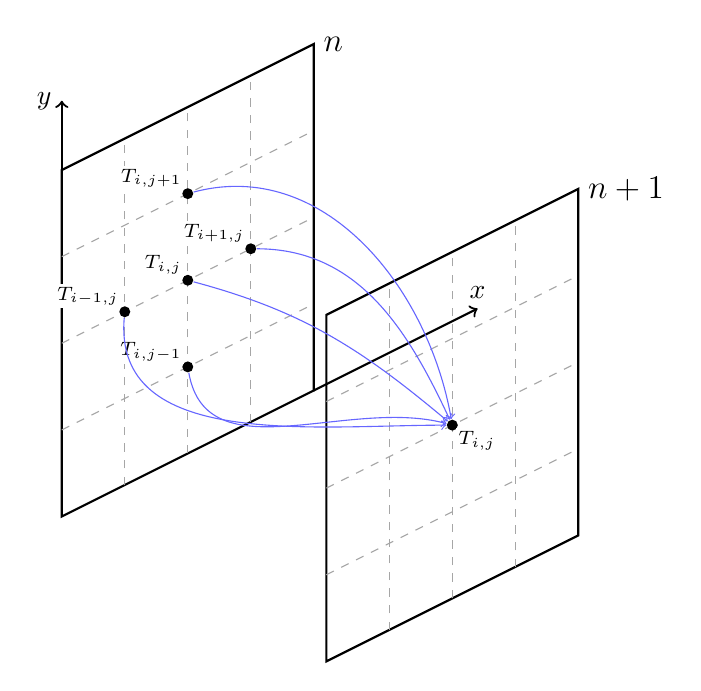
\begin{tikzpicture}[x={(0.8cm,0.4cm)}, y={(0cm,1.1cm)},
			tocka/.style={circle, fill, inner sep=1.4pt},
			oznaka/.style={font=\scriptsize, fill=white, inner sep=1pt},
			puscica/.style={->, blue!60, thin}]
			% ------------------ ravnina n ------------------
			\draw[thick] (0,0) -- (4,0) -- (4,4) -- (0,4) -- cycle;
			\foreach \k in {1,2,3} {
				\draw[dashed, gray!70] (\k,0) -- (\k,4);
				\draw[dashed, gray!70] (0,\k) -- (4,\k);
			}
			\node[right] at (4,4) {\large $n$};
			\draw[->, thick] (0,4) -- (0,4.8) node[left] {$y$};
			% tocke na ravnini n
			\node[tocka] (C) at (2,2) {};
			\node[tocka] (W) at (1,2) {};
			\node[tocka] (E) at (3,2) {};
			\node[tocka] (S) at (2,1) {};
			\node[tocka] (N) at (2,3) {};
			\node[oznaka, above left=1pt] at (C) {$T_{i,j}$};
			\node[oznaka, above left=1pt] at (W) {$T_{i-1,j}$};
			\node[oznaka, above left=1pt] at (E) {$T_{i+1,j}$};
			\node[oznaka, above left=1pt] at (S) {$T_{i,j-1}$};
			\node[oznaka, above left=1pt] at (N) {$T_{i,j+1}$};
			% ------------------ ravnina n+1 ------------------
			\begin{scope}[shift={(4.2,-3.2)}]
				\draw[thick, fill=white] (0,0) -- (4,0) -- (4,4) -- (0,4) -- cycle;
				\foreach \k in {1,2,3} {
					\draw[dashed, gray!70] (\k,0) -- (\k,4);
					\draw[dashed, gray!70] (0,\k) -- (4,\k);
				}
				\node[right] at (4,4) {\large $n+1$};
				\node[tocka] (C1) at (2,2) {};
				\node[oznaka, below right=1pt] at (C1) {$T_{i,j}$};
			\end{scope}
			% os x
			\draw[->, thick] (4,0) -- (6.6,0) node[above] {$x$};
			% ------------------ puscice ------------------
			\draw[puscica] (N) to[out=15,  in=100] (C1);
			\draw[puscica] (E) to[out=0,   in=115] (C1);
			\draw[puscica] (C) to[out=-15, in=140] (C1);
			\draw[puscica] (S) to[out=-80, in=165] (C1);
			\draw[puscica] (W) to[out=-95, in=180] (C1);
		\end{tikzpicture}
		\caption{Eksplicitna shema: vrednost $T_{i,j}$ na časovnem nivoju $n+1$ izračunamo iz petih vrednosti na nivoju $n$.}
		\label{fig:shema}
	\end{figure}
	
	% =====================================================================
	\subsection{Robni pogoji in navidezna vozlišča}
	
	Vsakič, ko dosežemo točko, ki je v interakciji z robom domene, apliciramo robne pogoje. V primeru Dirichletovih pogojev enostavno nastavimo zahtevano temperaturo v točki. Če je na robu Neumannov pogoj, ga aproksimiramo s pomočjo centralnih končnih diferenc. Neumannov robni pogoj določi odvod v smeri, pravokotni na rob domene. Na primer za pogoja
	\begin{align*}
		\frac{\partial T}{\partial y} &= q_y \quad \text{na spodnjem robu}, &
		\frac{\partial T}{\partial x} &= q_x \quad \text{na desnem robu}
	\end{align*}
	nastavimo $q_x = q_y = 0$ (izolacija). Kar diskretiziramo kot
	\begin{align*}
		\frac{T^n_{i,1} - T^n_{i,-1}}{2\Delta y} &= 0, &
		\frac{T^n_{N_x+1,j} - T^n_{N_x-1,j}}{2\Delta x} &= 0,
	\end{align*}
	kar poenostavimo v
	\begin{equation}
		T^n_{i,-1} = T^n_{i,1}, \qquad T^n_{N_x+1,j} = T^n_{N_x-1,j}.
		\label{eq:navidezne}
	\end{equation}
	Za točke na robu z Neumannovim pogojem vrednosti temperature ne poznamo, zato jih izračunamo s posodobitveno formulo kot notranje točke. Ta pa potrebuje tudi točke izven mreže, npr.\ $(i, -1)$ ali $(N_x+1, j)$, ki jih v naši mreži ni. Zato jih dodamo v mrežo kot t.~i.\ navidezna vozlišča, njihove vrednosti pa določimo iz Neumannovega pogoja~\eqref{eq:navidezne}.
	
	% =====================================================================
	\subsection{Stabilnost}
	
	Metoda ima maksimalen časovni korak, ki ga lahko uporabimo pri računanju. V primeru, da ga presežemo, postane metoda nestabilna in dobimo napačne rezultate. Pogoj stabilnosti v dveh dimenzijah zapišemo kot
	\begin{equation}
		D\,\Delta t \left(\frac{1}{\Delta x^2} + \frac{1}{\Delta y^2}\right) \leq \frac{1}{2}.
		\label{eq:stabilnost}
	\end{equation}
	Iz njega v implementaciji določimo časovni korak kot
	\begin{equation}
		\Delta t = \frac{1}{2D\left(\frac{1}{\Delta x^2} + \frac{1}{\Delta y^2}\right)}.
	\end{equation}
	
	% =====================================================================
	\subsection{Ustavitveni pogoj}
	
	Metodo izvajamo, dokler ni izpolnjen pogoj
	\begin{equation}
		\max_{i,j} \left| T^{n+1}_{i,j} - T^n_{i,j} \right| < \text{tol},
		\label{eq:ustavitev}
	\end{equation}
	kjer je $\text{tol}$ toleranca.
	
	\newpage
	
	\section{Implementacija}
	
	% =====================================================================
	\subsection{Orodja}
	
	Numerično metodo implementiramo v jeziku Fortran, kjer smo pri prevajanju uporabili zastavico za optimizacijo \texttt{-O2} in dvojno natančnost pri realnih številih. Na podlagi podatkov, generiranih s programom v Fortranu, ustvarimo diagrame s pomočjo jezika Python. Celotna izvorna koda je dostopna na \url{https://github.com/abrodar/2D-enacba-prenosa-toplote}.
	
	% =====================================================================
	\subsection{Vhodni parametri}
	
	Glavni vhodni parametri programa so sledeči. Najprej določimo dolžino $L$ in višino $H$ pravokotne domene. V obeh primerih je vrednost enaka ena. Nato določimo število točk v smeri $x$ in $y$ s parametroma $n_x$ in $n_y$. Pri vsaki meritvi je veljal pogoj $n_x = n_y$. Potrebno je določiti tudi vrednost toplotne difuzivnosti $D$ in tolerance $\text{tol}$. Pri parametrih $n_x$ (in s tem $n_y$), $D$ in $\text{tol}$ testiramo več različnih vrednosti.
	
	Korak $\Delta x$ (analogno $\Delta y$) določimo tako, da dolžino $L$ delimo s številom vseh enako velikih intervalov med $n_x$ točkami. Teh je za ena manj kot točk, torej
	\begin{equation}
		\Delta x = \frac{L}{n_x - 1}.
	\end{equation}
	Podobno velja za višino, kjer je
	\begin{equation}
		\Delta y = \frac{H}{n_y - 1}.
	\end{equation}
	Kot smo opisali na koncu prejšnjega poglavja, $\Delta t$ določimo na podlagi pogoja stabilnosti~\eqref{eq:stabilnost}.
	
	Pogoj stabilnosti preverjamo tako, da najprej definiramo konstanti
	\begin{equation}
		c_1 = \frac{D\,\Delta t}{\Delta x^2}, \qquad c_2 = \frac{D\,\Delta t}{\Delta y^2},
	\end{equation}
	nato pa z izvajanjem nadaljujemo le, če velja $c_1 + c_2 \leq \frac{1}{2}$.
	
	% =====================================================================
	\subsection{Pomnilniška razporeditev}
	
	Fizikalni problem ima dve dimenziji, zato hranimo temperature v dveh dimenzijah, in sicer v dvodimenzionalni tabeli. Podatke shranimo tako, da se ujemajo s fizikalno orientacijo problema. Vrstice tabele predstavljajo koordinato $y$, stolpci tabele pa koordinato $x$. Vrstici z indeksoma $0$ in $n_y + 1$ sta namenjeni navideznim vozliščem. Torej prej definirane koordinate $0, 1, \dots, N_x$ v programu predstavimo z indeksi $1, 2, \dots, n_x$ (analogno velja za smer $y$). Na primer, prvi testni primer predstavimo na sliki~\ref{fig:tabela1}.
	
	\begin{figure}[htbp]
		\centering
		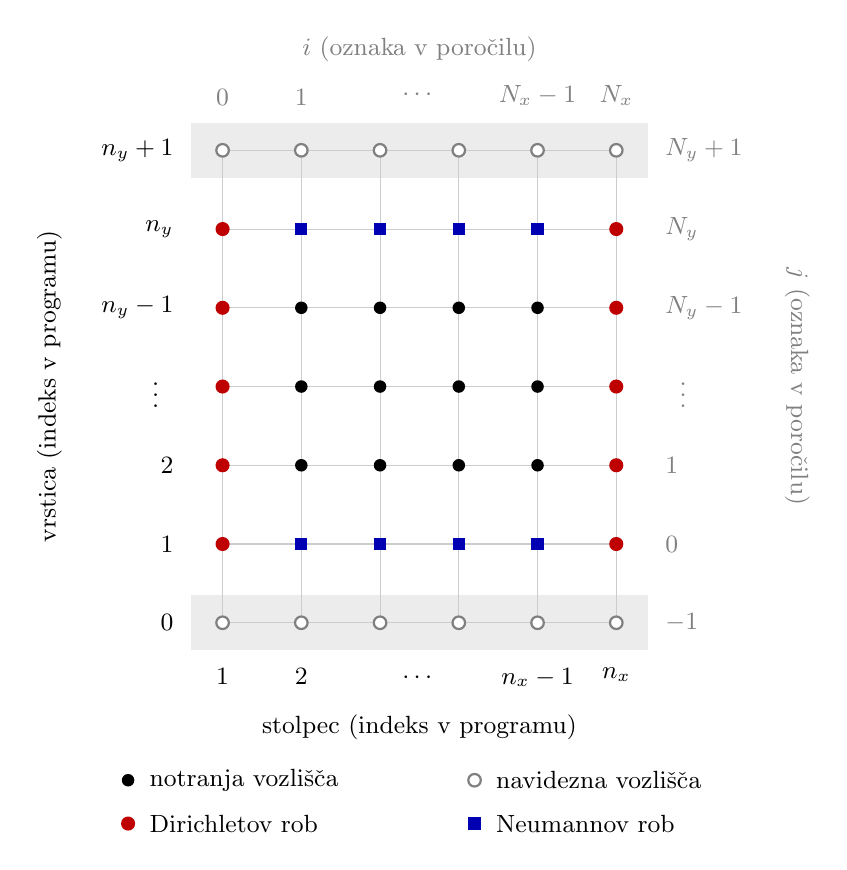
\begin{tikzpicture}[scale=1.0,
			notranje/.style={circle, fill=black, inner sep=1.6pt},
			dirichlet/.style={circle, fill=red!75!black, inner sep=1.8pt},
			neumann/.style={rectangle, fill=blue!70!black, inner sep=2.2pt},
			navidezno/.style={circle, draw=gray, fill=white, thick, inner sep=1.6pt},
			koda/.style={font=\small},
			porocilo/.style={font=\small, gray}]
			% pas navideznih vozlisc
			\fill[gray!15] (-0.4, -0.35) rectangle (5.4, 0.35);
			\fill[gray!15] (-0.4, 5.65) rectangle (5.4, 6.35);
			% mrezne crte
			\foreach \a in {0,...,5} \draw[gray!40] (\a, 0) -- (\a, 6);
			\foreach \b in {0,...,6} \draw[gray!40] (0, \b) -- (5, \b);
			% vozlisca
			\foreach \a in {0,...,5} {
				\node[navidezno] at (\a, 0) {};
				\node[navidezno] at (\a, 6) {};
				\foreach \b in {1,...,5} {
					\pgfmathtruncatemacro{\dir}{(\a==0) || (\a==5)}
					\pgfmathtruncatemacro{\neu}{(\b==1) || (\b==5)}
					\ifnum\dir=1
					\node[dirichlet] at (\a, \b) {};
					\else\ifnum\neu=1
					\node[neumann] at (\a, \b) {};
					\else
					\node[notranje] at (\a, \b) {};
					\fi\fi
				}
			}
			% indeksi v programu (spodaj in levo)
			\foreach \a/\lab in {0/{1}, 1/{2}, 4/{n_x-1}, 5/{n_x}}
			\node[koda, below] at (\a, -0.45) {$\lab$};
			\node[koda] at (2.5, -0.7) {$\cdots$};
			\foreach \b/\lab in {0/{0}, 1/{1}, 2/{2}, 4/{n_y-1}, 5/{n_y}, 6/{n_y+1}}
			\node[koda, left] at (-0.5, \b) {$\lab$};
			\node[koda] at (-0.85, 3) {$\vdots$};
			\node[koda, below] at (2.5, -1.05) {stolpec (indeks v programu)};
			\node[koda, rotate=90] at (-2.2, 3) {vrstica (indeks v programu)};
			% indeksi v porocilu (zgoraj in desno)
			\foreach \a/\lab in {0/{0}, 1/{1}, 4/{N_x-1}, 5/{N_x}}
			\node[porocilo, above] at (\a, 6.45) {$\lab$};
			\node[porocilo] at (2.5, 6.7) {$\cdots$};
			\foreach \b/\lab in {0/{-1}, 1/{0}, 2/{1}, 4/{N_y-1}, 5/{N_y}, 6/{N_y+1}}
			\node[porocilo, right] at (5.5, \b) {$\lab$};
			\node[porocilo] at (5.85, 3) {$\vdots$};
			\node[porocilo, above] at (2.5, 7.0) {$i$ (oznaka v poročilu)};
			\node[porocilo, rotate=-90] at (7.3, 3) {$j$ (oznaka v poročilu)};
			% legenda
			\begin{scope}[shift={(-1.2, -2.0)}]
				\node[notranje] at (0, 0) {};       \node[right, font=\small] at (0.15, 0) {notranja vozlišča};
				\node[navidezno] at (4.4, 0) {};    \node[right, font=\small] at (4.55, 0) {navidezna vozlišča};
				\node[dirichlet] at (0, -0.55) {};  \node[right, font=\small] at (0.15, -0.55) {Dirichletov rob};
				\node[neumann] at (4.4, -0.55) {};  \node[right, font=\small] at (4.55, -0.55) {Neumannov rob};
			\end{scope}
		\end{tikzpicture}
		\caption{Razporeditev tabele \texttt{T(0:ny+1, 1:nx)} za testni primer~1: vrstice ustrezajo smeri $y$, stolpci smeri $x$. Spodaj in levo so indeksi v programu, zgoraj in desno (sivo) pripadajoče oznake iz razdelka~2.}
		\label{fig:tabela1}
	\end{figure}
	
	% =====================================================================
	\subsection{Inicializacija}
	
	V obeh testnih primerih najprej nastavimo vse točke na temperaturo $50$. Nato v prvem testnem primeru nastavimo levi rob na temperaturo $100$ in desni rob na temperaturo $0$. Pri drugem testnem primeru nastavimo levi in desni rob na temperaturo $0$ ter spodnji rob po formuli
	\begin{equation}
		T(x, 0) = 100 \sin(\pi x).
	\end{equation}
	
	% =====================================================================
	\subsection{Glavna zanka}
	
	V tem razdelku podamo psevdokodo glavne zanke programa (algoritem~\ref{alg:zanka}). Psevdokoda uporabi indeks $i$ za smer $x$ in $j$ za smer $y$. V programu zunanja zanka teče po stolpcih, notranja pa po vrsticah znotraj stolpca, ker Fortran hrani dvodimenzionalno tabelo stolpec za stolpcem, tj.\ \texttt{T(0,1)}, \texttt{T(1,1)}, \texttt{T(2,1)}, \dots, \texttt{T(0,2)}, \texttt{T(1,2)}, \dots\ Na ta način zaporedno dostopamo do sosednjih pomnilniških lokacij v predpomnilniku.
	
	\begin{algorithm}[htbp]
		\caption{Glavna zanka eksplicitne sheme (testni primer~1).}
		\label{alg:zanka}
		\begin{algorithmic}[1]
			\Require začetno polje $T^{\text{prej}}$ z robnimi vrednostmi, $c_1$, $c_2$, $\text{tol}$, $n_t$
			\Ensure ustaljeno temperaturno polje $T$
			\For{$k = 1, \dots, n_t$}
			\For{$i = 2, \dots, n_x - 1$} \Comment{vsi stolpci razen Dirichletovih}
			\For{$j = 1, \dots, n_y$} \Comment{vključno z Neumannovima vrsticama}
			\State $T_{i,j} \gets T^{\text{prej}}_{i,j} + c_1\left(T^{\text{prej}}_{i+1,j} - 2T^{\text{prej}}_{i,j} + T^{\text{prej}}_{i-1,j}\right)$
			\Statex \hspace{\algorithmicindent}\hspace{\algorithmicindent}\hspace{\algorithmicindent}\hspace{\algorithmicindent}\hspace{1.2cm}$+\, c_2\left(T^{\text{prej}}_{i,j+1} - 2T^{\text{prej}}_{i,j} + T^{\text{prej}}_{i,j-1}\right)$
			\EndFor
			\EndFor
			\State $T_{i,0} \gets T_{i,2}$, \quad $T_{i,n_y+1} \gets T_{i,n_y-1}$ \Comment{navidezna vozlišča}
			\State $\delta \gets \max_{i,j} \left| T_{i,j} - T^{\text{prej}}_{i,j} \right|$
			\If{$\delta < \text{tol}$}
			\State \textbf{ustavi} \Comment{ustaljeno stanje}
			\EndIf
			\State $T^{\text{prej}} \gets T$
			\EndFor
		\end{algorithmic}
	\end{algorithm}
	
	Algoritem~\ref{alg:zanka} velja za prvi testni primer. V drugem testnem primeru je spodnji rob Dirichletov, zato notranja zanka teče od $j = 2$ dalje, navidezna vozlišča pa potrebujemo le na zgornjem robu, kjer velja $T_{i,n_y+1} \gets T_{i,n_y-1}$.
	
	% =====================================================================
	\subsection{Izhod in napaka}
	
	Končno temperaturno porazdelitev $T$ zapišemo v datoteko s končnico \texttt{.data}. Obenem zabeležimo, pri katerem koraku je metoda konvergirala in kakšna je bila njena največja absolutna napaka
	\begin{equation}
		E = \max_{i,j} \left| T_{i,j} - T^{\text{točna}}_{i,j} \right|.
		\label{eq:napaka}
	\end{equation}
	\newpage
	
	\section{Rezultati}
	
	V tem razdelku prikažemo rezultate eksperimentov oz.\ izvajanja programa za oba testna primera.
	
	% =====================================================================
	\subsection{Testni primer 1: Linearni temperaturni profil}
	
	Na temperaturnem polju prvega testnega primera (slika~\ref{fig:kontura1}) opazimo enakomerno porazdeljene izoterme. Temperatura v domeni pada od leve proti desni. Izoterme so navpične oz.\ se temperatura vzdolž osi $y$ ne spreminja, tj.\ $\frac{\partial T}{\partial y} = 0$.
	
	V tabeli~\ref{tab:mreza1} spreminjamo velikost mreže in spremljamo, kako se spreminjajo število korakov metode, njena največja absolutna napaka in čas izvajanja. Število korakov z gostejšo mrežo narašča. Ravno tako se povečata čas izvajanja in izmerjena napaka.
	
	\begin{figure}[htbp]
		\centering
		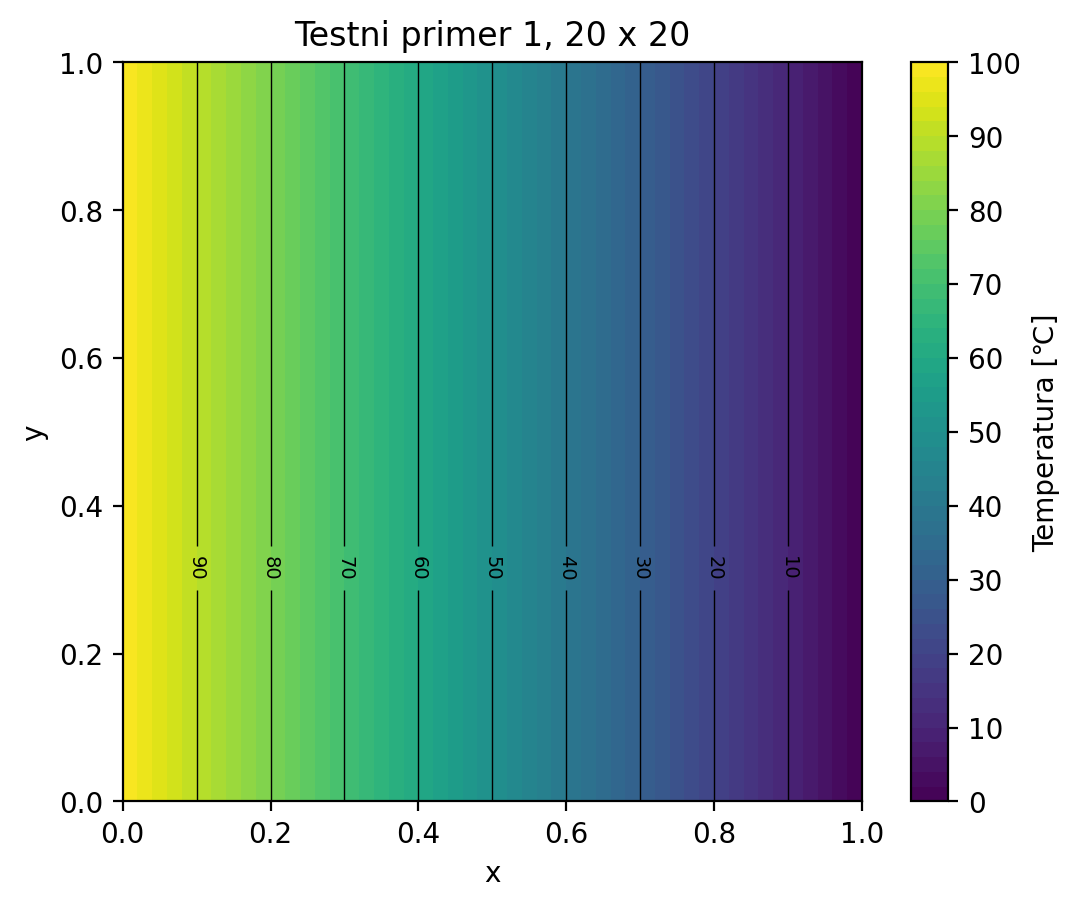
\includegraphics[width=0.7\textwidth]{slike/T_test1_contour_20x20.png}
		\caption{Testni primer~1: temperaturno polje v ustaljenem stanju na mreži $20 \times 20$.}
		\label{fig:kontura1}
	\end{figure}
	
	\begin{table}[htbp]
		\centering
		\begin{tabular}{lrrrr}
			\toprule
			$n_x = n_y$          & 10                       & 20                       & 50                       & 100                      \\
			\midrule
			št.\ korakov         & 234                      & 1002                     & 6223                     & 24020                    \\
			$E$                  & $6{,}84 \cdot 10^{-12}$ & $3{,}51 \cdot 10^{-11}$ & $2{,}43 \cdot 10^{-10}$ & $9{,}91 \cdot 10^{-10}$ \\
			čas izvajanja [s]    & 0{,}004                  & 0{,}008                  & 0{,}061                  & 0{,}415                  \\
			\bottomrule
		\end{tabular}
		\caption{Testni primer~1: vpliv gostote mreže ($D = 1$, $\text{tol} = 10^{-12}$, $n_t = 10^5$). $E$ je največja absolutna napaka~\eqref{eq:napaka}.}
		\label{tab:mreza1}
	\end{table}
	
	% =====================================================================
	\subsection{Testni primer 2: Dvodimenzionalna stacionarna rešitev}
	
	V drugem testnem primeru opazimo na sliki~\ref{fig:kontura2} najvišje temperature ob spodnjem robu domene. Izoterme imajo obliko ukrivljenih lokov. Večja kot je vrednost $y$, bolj ukrivljeni postanejo loki. Razmiki med njimi se z višino povečujejo. Temperatura z višino pada, hkrati pa je nižja tudi ob približevanju levemu ali desnemu robu.
	
	V tabeli~\ref{tab:mreza2} je razvidno, da se število korakov z več točkami v mreži povečuje enako kot pri prvem testnem primeru. Napaka se tokrat, v nasprotju s prvim primerom, zmanjšuje. Čas izvajanja metode pa še vedno narašča.
	
	\begin{figure}[htbp]
		\centering
		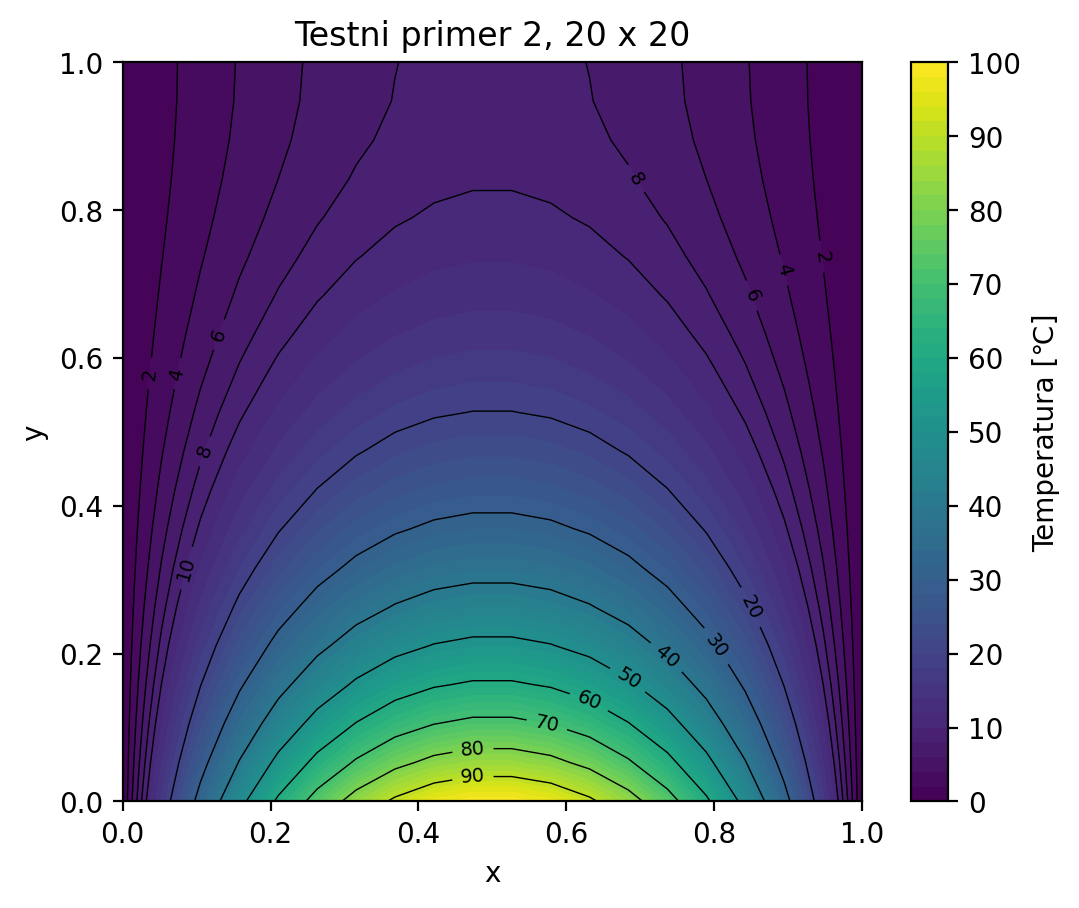
\includegraphics[width=0.7\textwidth]{slike/T_test2_contour_20x20.png}
		\caption{Testni primer~2: temperaturno polje v ustaljenem stanju na mreži $20 \times 20$.}
		\label{fig:kontura2}
	\end{figure}
	
	\begin{table}[htbp]
		\centering
		\begin{tabular}{lrrrr}
			\toprule
			$n_x = n_y$          & 10                       & 20                       & 50                       & 100                      \\
			\midrule
			št.\ korakov         & 738                      & 3140                     & 19450                    & 74960                    \\
			$E$                  & $3{,}87 \cdot 10^{-1}$  & $8{,}83 \cdot 10^{-2}$  & $1{,}34 \cdot 10^{-2}$  & $3{,}28 \cdot 10^{-3}$  \\
			čas izvajanja [s]    & 0{,}005                  & 0{,}014                  & 0{,}192                  & 1{,}366                  \\
			\bottomrule
		\end{tabular}
		\caption{Testni primer~2: vpliv gostote mreže ($D = 1$, $\text{tol} = 10^{-12}$, $n_t = 10^5$). $E$ je največja absolutna napaka~\eqref{eq:napaka}.}
		\label{tab:mreza2}
	\end{table}
	
	% =====================================================================
	\subsection{Vpliv toplotne difuzivnosti $D$}
	
	Izvedemo poseben eksperiment za preverjanje vpliva toplotne difuzivnosti $D$ na rešitev. Testiramo oba testna primera, in sicer pri naslednjih nastavitvah parametrov: $n_x = n_y = 20$, $\text{tol} = 10^{-12}$, $n_t = 10^5$. Eksperiment izvedemo za vrednosti parametra $D$: $0{,}1$, $1$, $10$ in $100$.
	
	Na podlagi teorije pričakujemo tri opažanja. Prvič, parameter $D$ naj ne bi vplival na ustaljeno stanje. Za ustaljeno stanje velja $\frac{\partial T}{\partial t} = 0$. Če to vstavimo v toplotno enačbo, dobimo $0 = \nabla^2 T$, kjer smo lahko enačbo delili z $D$. Ustaljeno stanje je torej neodvisno od toplotne difuzivnosti. Nadalje opazimo, da bi moralo število korakov ostati enako. V zgoraj definiranih členih $c_1$ in $c_2$, ki ju uporabljamo v glavni zanki, se namreč $D$ iz produkta $D\,\Delta t$ pokrajša z $D$ v imenovalcu izraza za $\Delta t$:
	\begin{equation}
		D\,\Delta t = D \cdot \frac{1}{2D\left(\frac{1}{\Delta x^2} + \frac{1}{\Delta y^2}\right)} = \frac{1}{2\left(\frac{1}{\Delta x^2} + \frac{1}{\Delta y^2}\right)}.
	\end{equation}
	Kot tretje je razvidno, da z večjim $D$ zmanjšamo (fizikalni) čas. Ob upoštevanju diskretizacije ga definiramo kot $t = k\,\Delta t$. Če vanj vstavimo $\Delta t$, dobimo $t \propto \frac{k}{D}$.
	
	V obeh testnih primerih v tabelah~\ref{tab:D1} in~\ref{tab:D2} opazimo, da se teorija udejanji v praksi. Število korakov in napaka v obeh primerih ostaneta enaka pri vseh vrednostih $D$. Časovni korak se zmanjšuje za faktor $10$, ko $D$ povečamo za enak faktor. Ravno tako se po enakem pravilu zmanjšuje (fizikalni) čas.
	
	\begin{table}[htbp]
		\centering
		\begin{tabular}{lrrrr}
			\toprule
			$D$                  & 0{,}1                    & 1                        & 10                       & 100                      \\
			\midrule
			št.\ korakov $k$     & 1002                     & 1002                     & 1002                     & 1002                     \\
			$E$                  & $3{,}51 \cdot 10^{-11}$ & $3{,}51 \cdot 10^{-11}$ & $3{,}51 \cdot 10^{-11}$ & $3{,}51 \cdot 10^{-11}$ \\
			čas izvajanja [s]    & 0{,}007                  & 0{,}006                  & 0{,}007                  & 0{,}007                  \\
			$\Delta t$           & $6{,}93 \cdot 10^{-3}$  & $6{,}93 \cdot 10^{-4}$  & $6{,}93 \cdot 10^{-5}$  & $6{,}93 \cdot 10^{-6}$  \\
			$t = k\,\Delta t$    & $6{,}94$                 & $6{,}94 \cdot 10^{-1}$  & $6{,}94 \cdot 10^{-2}$  & $6{,}94 \cdot 10^{-3}$  \\
			\bottomrule
		\end{tabular}
		\caption{Testni primer~1: vpliv toplotne difuzivnosti $D$ ($n_x = n_y = 20$, $\text{tol} = 10^{-12}$, $n_t = 10^5$).}
		\label{tab:D1}
	\end{table}
	
	\begin{table}[htbp]
		\centering
		\begin{tabular}{lrrrr}
			\toprule
			$D$                  & 0{,}1                    & 1                        & 10                       & 100                      \\
			\midrule
			št.\ korakov $k$     & 3140                     & 3140                     & 3140                     & 3140                     \\
			$E$                  & $8{,}83 \cdot 10^{-2}$  & $8{,}83 \cdot 10^{-2}$  & $8{,}83 \cdot 10^{-2}$  & $8{,}83 \cdot 10^{-2}$  \\
			čas izvajanja [s]    & 0{,}013                  & 0{,}013                  & 0{,}011                  & 0{,}013                  \\
			$\Delta t$           & $6{,}93 \cdot 10^{-3}$  & $6{,}93 \cdot 10^{-4}$  & $6{,}93 \cdot 10^{-5}$  & $6{,}93 \cdot 10^{-6}$  \\
			$t = k\,\Delta t$    & $2{,}17 \cdot 10^{1}$   & $2{,}17$                 & $2{,}17 \cdot 10^{-1}$  & $2{,}17 \cdot 10^{-2}$  \\
			\bottomrule
		\end{tabular}
		\caption{Testni primer~2: vpliv toplotne difuzivnosti $D$ ($n_x = n_y = 20$, $\text{tol} = 10^{-12}$, $n_t = 10^5$).}
		\label{tab:D2}
	\end{table}
	
	% =====================================================================
	\subsection{Stabilnost}
	
	Zadnji izveden eksperiment se ukvarja s stabilnostjo metode. V vsaki izvedbi spreminjamo parameter $s = c_1 + c_2$, uporabljen v implementaciji pri časovnem koraku
	\begin{equation}
		\Delta t = \frac{s}{D\left(\frac{1}{\Delta x^2} + \frac{1}{\Delta y^2}\right)}.
	\end{equation}
	
	V prvem testnem primeru metoda pri vrednostih $s$ od $0{,}25$ do $0{,}6$ vedno konvergira in ostane stabilna (tabela~\ref{tab:stabilnost1}). Ker nas je zanimalo, kdaj postane nestabilna, smo eksperiment izvedli tudi pri večjih vrednostih in izkaže se, da je meja $s = 1$: pri $s = 1$ metoda konvergira v $2005$ korakih, pri $s = 1{,}1$ pa postane nestabilna že v $25.$~koraku. Ta vrednost ustreza meji pri enodimenzionalni različici problema. Nad to vrednostjo metoda ne konvergira več.
	
	V drugem testnem primeru je ta meja $s = 0{,}5$. Že pri $s = 0{,}51$ metoda ne konvergira in v $735.$~koraku dosežemo skrajno vrednost $-0{,}0225$ (tabela~\ref{tab:stabilnost2}).
	
	\begin{table}[htbp]
		\centering
		\begin{tabular}{lrrrrrr}
			\toprule
			$s$                  & 0{,}25  & 0{,}45  & 0{,}5   & 0{,}51  & 0{,}55  & 0{,}6   \\
			\midrule
			št.\ korakov         & 1965    & 1110    & 1002    & 983     & 913     & 838     \\
			čas izvajanja [s]    & 0{,}013 & 0{,}007 & 0{,}009 & 0{,}009 & 0{,}009 & 0{,}009 \\
			konvergenca          & da      & da      & da      & da      & da      & da      \\
			\bottomrule
		\end{tabular}
		\caption{Testni primer~1: vpliv faktorja $s = c_1 + c_2$ na stabilnost ($D = 1$, $n_x = n_y = 20$, $\text{tol} = 10^{-12}$, $n_t = 10^5$).}
		\label{tab:stabilnost1}
	\end{table}
	
	\begin{table}[htbp]
		\centering
		\begin{tabular}{lrrrrrr}
			\toprule
			$s$                  & 0{,}25  & 0{,}45  & 0{,}5   & 0{,}51                   & 0{,}55                   & 0{,}6                    \\
			\midrule
			št.\ korakov         & 6130    & 3477    & 3140    & 735                      & 56                       & 26                       \\
			skrajna vrednost     & --      & --      & --      & $-0{,}0225$              & $-0{,}159$               & $-0{,}790$               \\
			čas izvajanja [s]    & 0{,}028 & 0{,}020 & 0{,}017 & 0{,}008                  & 0{,}005                  & 0{,}005                  \\
			konvergenca          & da      & da      & da      & ne                       & ne                       & ne                       \\
			\bottomrule
		\end{tabular}
		\caption{Testni primer~2: vpliv faktorja $s = c_1 + c_2$ na stabilnost ($D = 1$, $n_x = n_y = 20$, $\text{tol} = 10^{-12}$, $n_t = 10^5$). Pri nestabilnih primerih je navedeno število korakov do zaznane nestabilnosti in vrednost temperature, ki je prvič padla izven intervala $[0, 100]$.}
		\label{tab:stabilnost2}
	\end{table}
	
	\newpage
	\section{Analiza napak in zaključek}
	
	V tem razdelku analiziramo vire napak rešitve, red konvergence in vpliv tolerance. Na koncu povzamemo glavne ugotovitve naloge.
	
	% =====================================================================
	\subsection{Viri napake}
	
	Skupno napako sestavljata dva dela, in sicer napaka mreže in napaka ustavitve:
	\begin{equation}
		E = E_{\text{mreža}} + E_{\text{ustavitev}}.
		\label{eq:viri}
	\end{equation}
	
	Napako mreže imamo zaradi aproksimacije odvodov s končnimi diferencami. Ta se zmanjšuje sorazmerno z $\Delta x^2$, kar sledi iz napake centralne diference~\eqref{eq:drugi_odvod}. Napaka ustavitve izvira iz uporabljenega ustavitvenega pogoja. Program ustavimo, ko je sprememba na časovni korak manjša od tolerance, vendar se rešitev še vedno približuje ustaljenemu stanju. Naj bo $d_k$ največja razdalja med rešitvijo v $k$-tem časovnem koraku in ustaljenim stanjem. Proti koncu računanja se ta razdalja v vsakem časovnem koraku zmanjša za približno enak faktor $\rho < 1$:
	\begin{equation}
		d_{k+1} = \rho\, d_k.
	\end{equation}
	Sprememba rešitve v enem koraku je zato
	\begin{equation}
		d_k - d_{k+1} = (1 - \rho)\, d_k.
	\end{equation}
	Računanje ustavimo, ko je sprememba manjša od $\text{tol}$, torej ko velja $(1-\rho)\,d_k < \text{tol}$. Razdalja do ustaljenega stanja, ki ostane, je tedaj
	\begin{equation}
		E_{\text{ustavitev}} \approx \frac{\text{tol}}{1 - \rho}.
		\label{eq:ustavitev_napaka}
	\end{equation}
	Tabela~\ref{tab:primer_ustavitev} prikazuje primer za $\rho = 0{,}9$, $d_1 = 10$ in $\text{tol} = 0{,}1$. Računanje se ustavi pri $d \approx 0{,}89$, kar je skoraj desetkrat več od tolerance in se ujema z oceno $\text{tol}/(1-\rho) = 1$.
	
	\begin{table}[htbp]
		\centering
		\begin{tabular}{rrl}
			\toprule
			$d_k$     & $d_{k-1} - d_k$ & \\
			\midrule
			$10$      &                  & \\
			$9$       & $1$              & \\
			$8{,}1$   & $0{,}9$          & \\
			$\vdots$  & $\vdots$         & \\
			$1{,}094$ & $0{,}122$        & \\
			$0{,}985$ & $0{,}109$        & \\
			$0{,}886$ & $0{,}099$        & $< \text{tol}$, ustavitev \\
			\bottomrule
		\end{tabular}
		\caption{Primer ustavitve pri $\rho = 0{,}9$ in $\text{tol} = 0{,}1$.}
		\label{tab:primer_ustavitev}
	\end{table}
	
	Napaka zaradi ustavitve je odvisna tudi od mreže. Recimo, da se rešitev v realnih fizikalnih razmerah vsako sekundo približa ustaljenemu stanju za $5\,\%$ preostale razdalje. Vsak korak programa se v času premakne naprej za $\Delta t$, zato je delež razdalje, ki ga opravimo v enem koraku, odvisen od dolžine koraka $\Delta t$. Pri $\Delta t = 1\,\text{s}$ je torej $1-\rho = 5\,\%$ oz.\ $\rho = 0{,}95$. Če korak zmanjšamo na $\Delta t = 0{,}25\,\text{s}$, je $1-\rho = 1{,}25\,\%$ oz.\ $\rho = 0{,}9875$. Krajši korak pokrije manj časa in zato opravi manj razdalje:
	\begin{equation}
		1 - \rho \approx \lambda\,\Delta t,
	\end{equation}
	kjer je $\lambda$ hitrost približevanja ustaljenemu stanju (delež preostale razdalje na enoto časa). Ta je odvisna le od fizikalnega problema in ne od mreže.
	
	Iz pogoja stabilnosti~\eqref{eq:stabilnost} pri $\Delta x = \Delta y$ sledi
	\begin{equation}
		\Delta t = \frac{\Delta x^2}{4D}.
	\end{equation}
	Če korak mreže $\Delta x$ razpolovimo, se $\Delta t$ zmanjša za faktor $4$. Za enak faktor se zmanjša tudi $1-\rho$, napaka zaradi ustavitve $\text{tol}/(1-\rho)$ pa se zato poveča za faktor $4$. V splošnem torej velja
	\begin{equation}
		E_{\text{ustavitev}} \approx \frac{\text{tol}}{1-\rho} \propto \frac{\text{tol}}{\Delta x^2}.
		\label{eq:ustavitev_mreza}
	\end{equation}
	
	Podobno kot za temperaturo v prejšnjem razdelku tokrat ustvarimo diagram, ki prikazuje polje napake za oba testna primera (slika~\ref{fig:napaka}). Pri obeh opazimo, da je napaka na robovih z Dirichletovimi pogoji enaka nič. To sta pri prvem primeru levi in desni rob, pri drugem pa levi, desni in spodnji rob. V prvem testnem primeru so napake zelo majhne, reda velikosti $10^{-11}$. Na levi polovici diagrama rešitev napoveduje nižje temperature od dejanskih, na desni polovici pa višje. Na diagramu drugega testnega primera so vse napake pozitivne oz.\ je izračunana temperatura povsod višja od točne. Največje napake se pojavijo v sredini diagrama in se postopoma zmanjšujejo, ko se približujemo robovom domene. Na zgornjem robu, kjer imamo Neumannov robni pogoj, je napaka v nasprotju z ostalimi robovi še vedno prisotna.
	
	\begin{figure}[htbp]
		\centering
		\begin{minipage}{0.48\textwidth}
			\centering
			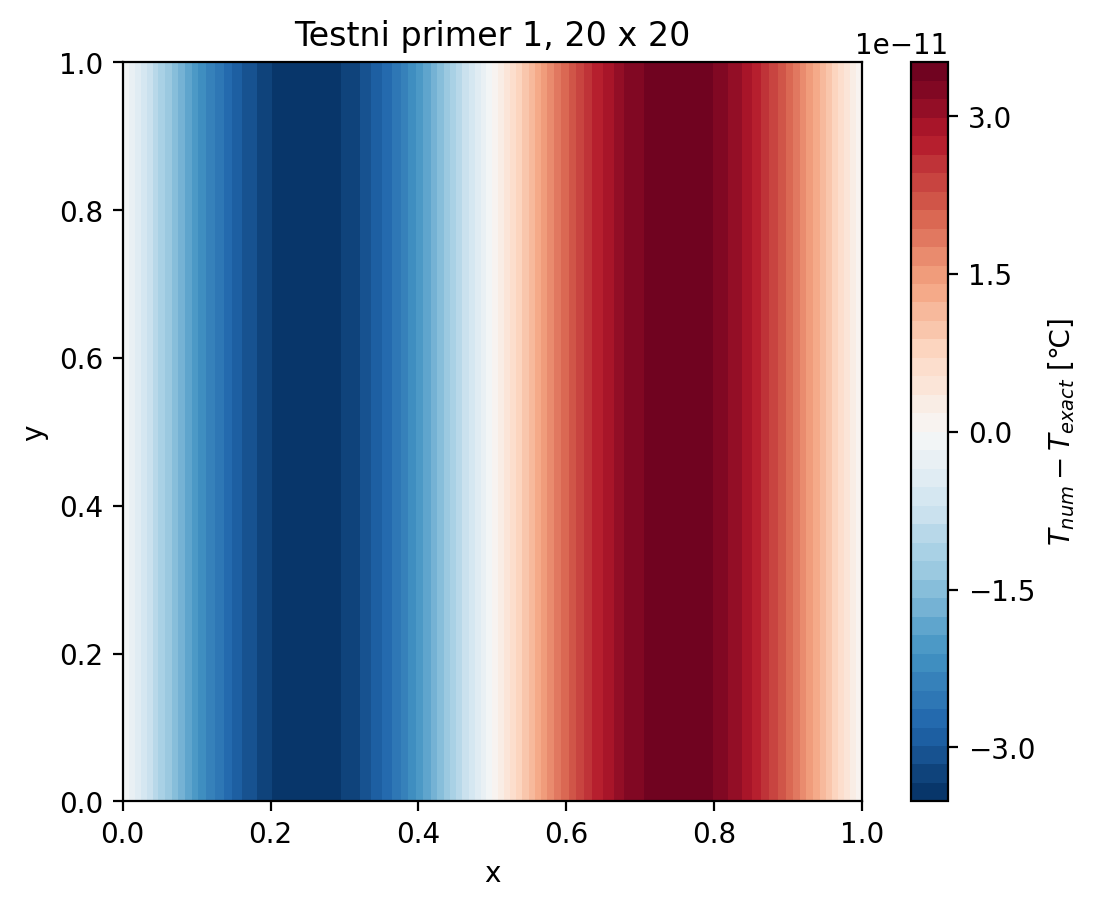
\includegraphics[width=\textwidth]{slike/testcase1_errfield_20x20.png}
			\\ (a) Testni primer~1
		\end{minipage}
		\hfill
		\begin{minipage}{0.48\textwidth}
			\centering
			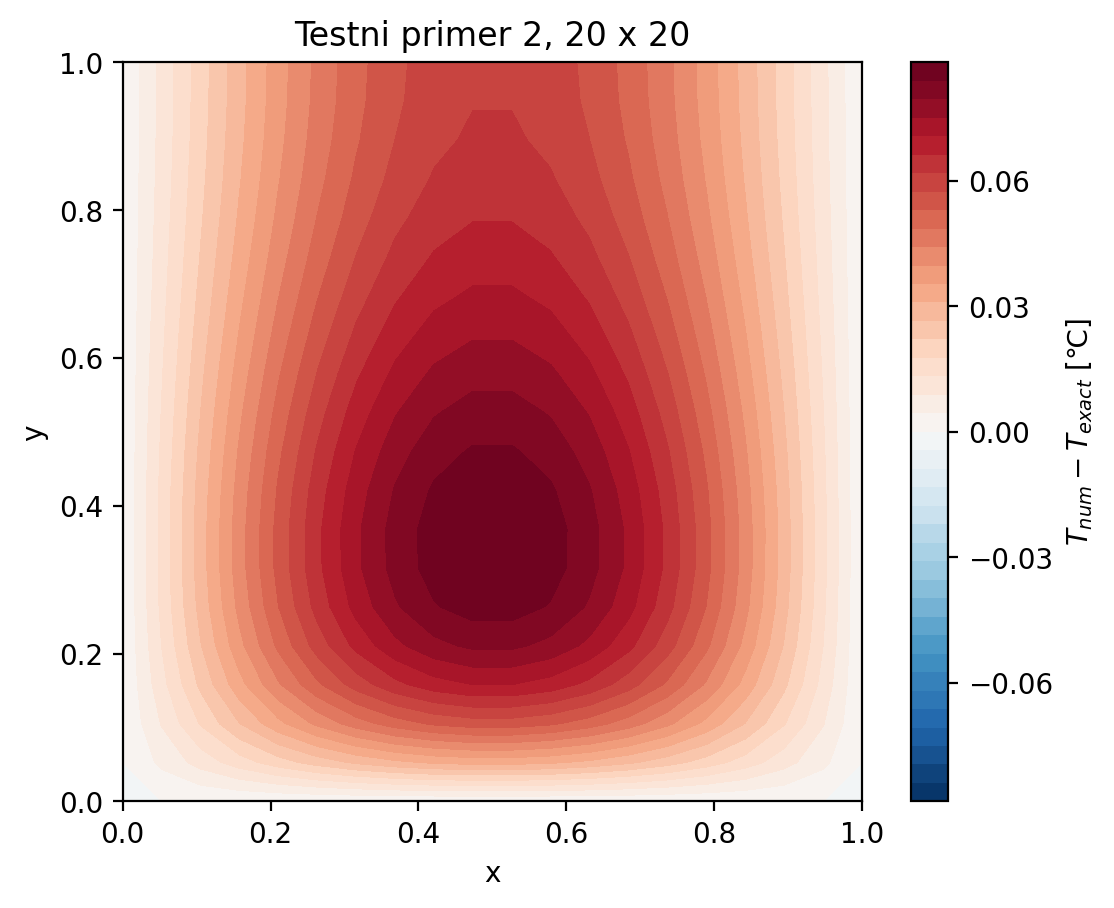
\includegraphics[width=\textwidth]{slike/testcase2_errfield_20x20.png}
			\\ (b) Testni primer~2
		\end{minipage}
		\caption{Polje napake $T_{\text{num}} - T_{\text{točna}}$ na mreži $20 \times 20$.}
		\label{fig:napaka}
	\end{figure}
		\FloatBarrier
	% =====================================================================
	
	\subsection{Red konvergence}
	
	Predpostavimo, da je napaka mreže sorazmerna s potenco koraka mreže:
	\begin{equation}
		E \approx C\,\Delta x^p,
	\end{equation}
	kjer je $p$ red konvergence, konstanta $C$ pa je odvisna od točne rešitve in ne od mreže.
	
	Za centralno diferenco je $p = 2$~\eqref{eq:drugi_odvod}. Poglejmo, kaj se zgodi z napako, če korak mreže razpolovimo. Na mreži s korakom $\Delta x$ je napaka $E' = C\,\Delta x^2$, na mreži s korakom $\Delta x/2$ pa
	\begin{equation}
		E'' = C\left(\frac{\Delta x}{2}\right)^2 = C\,\frac{\Delta x^2}{4} = \frac{E'}{4}.
	\end{equation}
	Ob razpolovitvi koraka mreže se napaka torej zmanjša za faktor $4$.
	
	V splošnem red konvergence določimo iz napak na dveh mrežah s koraki $\Delta x_1$ in $\Delta x_2$:
	\begin{equation}
		E_1 \approx C\,\Delta x_1^p, \qquad E_2 \approx C\,\Delta x_2^p.
	\end{equation}
	Enačbi delimo in konstanta $C$ se pokrajša:
	\begin{equation}
		\frac{E_1}{E_2} = \frac{C\,\Delta x_1^p}{C\,\Delta x_2^p} = \left(\frac{\Delta x_1}{\Delta x_2}\right)^p.
	\end{equation}
	Enačbo logaritmiramo in izrazimo $p$:
	\begin{equation}
		p = \frac{\ln(E_1/E_2)}{\ln(\Delta x_1/\Delta x_2)}.
		\label{eq:red}
	\end{equation}
	
	S pomočjo formule~\eqref{eq:red} izračunamo $p$ za oba testna primera. Rezultati so podani v tabeli~\ref{tab:red}. V prvem testnem primeru je red konvergence približno $-2$, v drugem pa $2$.
	
	\begin{table}[htbp]
		\centering
		\begin{tabular}{lrrr}
			\toprule
			$n_x = n_y$     & $10 \to 20$ & $20 \to 50$ & $50 \to 100$ \\
			\midrule
			testni primer 1 & $-2{,}19$   & $-2{,}04$   & $-2{,}00$    \\
			testni primer 2 & $1{,}98$    & $1{,}99$    & $2{,}00$     \\
			\bottomrule
		\end{tabular}
		\caption{Izmerjeni red konvergence $p$ med zaporednima mrežama po enačbi~\eqref{eq:red}.}
		\label{tab:red}
	\end{table}
	
	V drugem testnem primeru se izmerjeni red konvergence z gostitvijo mreže približuje vrednosti $p = 2$ (tabela~\ref{tab:red}), kar se ujema s teoretično napako centralne diference $\mathcal{O}(\Delta x^2)$~\eqref{eq:drugi_odvod}. To potrjuje napoved Taylorjeve vrste iz razdelka~2 oz.\ koda ima točnost, ki jo metoda obljublja v teoriji.
	
	V prvem testnem primeru je izmerjeni red konvergence negativen in se približuje vrednosti $p = -2$. Negativen red pomeni, da napaka z gostitvijo mreže narašča. Ker je napaka mreže v tem primeru enaka nič, je izmerjena napaka v celoti napaka zaradi ustavitve, za katero velja $E_{\text{ustavitev}} \propto \text{tol}/\Delta x^2 = \text{tol}\cdot\Delta x^{-2}$~\eqref{eq:ustavitev_mreza}, torej $p = -2$. Naraščanje napake zato ni posledica diskretizacije, temveč ustavitvenega pogoja. To pojasni, zakaj smo v prejšnjem razdelku v tabeli~\ref{tab:mreza1} opazili naraščanje napake, medtem ko je v drugem testnem primeru (tabela~\ref{tab:mreza2}) napaka z gostejšo mrežo padala.
	
	% =====================================================================
	\subsection{Vpliv tolerance}
	
	V prvem testnem primeru (tabela~\ref{tab:tol1}) opazimo, da se napaka zmanjša približno za faktor $100$ vsakič, ko toleranco zmanjšamo za enak faktor. Kot smo omenili že prej, v tem primeru igra vlogo le napaka ustavitve.
	
	\begin{table}[htbp]
		\centering
		\begin{tabular}{rrrr}
			\toprule
			$\text{tol}$ & št.\ korakov & $E$                     & čas izvajanja [s] \\
			\midrule
			$10^{-2}$    & 163          & $3{,}57 \cdot 10^{-1}$  & 0{,}005           \\
			$10^{-4}$    & 331          & $3{,}54 \cdot 10^{-3}$  & 0{,}005           \\
			$10^{-6}$    & 499          & $3{,}51 \cdot 10^{-5}$  & 0{,}005           \\
			$10^{-8}$    & 666          & $3{,}58 \cdot 10^{-7}$  & 0{,}006           \\
			$10^{-10}$   & 834          & $3{,}54 \cdot 10^{-9}$  & 0{,}006           \\
			$10^{-12}$   & 1002         & $3{,}51 \cdot 10^{-11}$ & 0{,}007           \\
			\bottomrule
		\end{tabular}
		\caption{Testni primer~1: vpliv tolerance ($D = 1$, $n_x = n_y = 20$, $n_t = 10^5$).}
		\label{tab:tol1}
	\end{table}
	
	V drugem testnem primeru (tabela~\ref{tab:tol2}) opazimo, da se napaka od tolerance $10^{-6}$ naprej bistveno ne zmanjša. Z drugimi besedami, od tam naprej napaka mreže prevladuje nad napako ustavitve, ki postane zanemarljivo majhna.
	
	\begin{table}[htbp]
		\centering
		\begin{tabular}{rrrr}
			\toprule
			$\text{tol}$ & št.\ korakov & $E$                     & čas izvajanja [s] \\
			\midrule
			$10^{-2}$    & 451          & $1{,}22$                & 0{,}006           \\
			$10^{-4}$    & 989          & $9{,}47 \cdot 10^{-2}$  & 0{,}008           \\
			$10^{-6}$    & 1527         & $8{,}84 \cdot 10^{-2}$  & 0{,}008           \\
			$10^{-8}$    & 2064         & $8{,}83 \cdot 10^{-2}$  & 0{,}010           \\
			$10^{-10}$   & 2602         & $8{,}83 \cdot 10^{-2}$  & 0{,}010           \\
			$10^{-12}$   & 3140         & $8{,}83 \cdot 10^{-2}$  & 0{,}011           \\
			\bottomrule
		\end{tabular}
		\caption{Testni primer~2: vpliv tolerance ($D = 1$, $n_x = n_y = 20$, $n_t = 10^5$).}
		\label{tab:tol2}
	\end{table}
	
	V obeh primerih z manjšanjem tolerance povečamo število korakov, potrebnih do konvergence. Z izbiro pretirano nizke tolerance torej plačamo le z dodatnimi koraki (3140 namesto 1527), rezultat pa se pri tem ne izboljša. Če bi v tem primeru želeli manjšo napako, bi morali zgostiti mrežo, ne pa zmanjšati tolerance. Smiselna toleranca je torej tista, pri kateri je napaka ustavitve jasno manjša od napake mreže.
	
	\subsection{Zaključek}
	
	V projektni nalogi smo reševali dvodimenzionalno enačbo prenosa toplote z eksplicitno shemo (prema diferenca v času in centralna v prostoru) z navideznimi vozlišči za Neumannove pogoje. Metoda je bila zapisana v programskem jeziku Fortran in preverjena na dveh testnih primerih z znanimi rešitvami.
	
	Z vidika pravilnosti ugotovimo, da implementacija v drugem testnem primeru doseže red konvergence $p \approx 2$, kot smo napovedali s Taylorjevo vrsto. Napake metode imajo dva izvora. V prvem testnem primeru prevladuje napaka ustavitve, v drugem pa napaka mreže. Pri preučevanju parametra $D$ opazimo, da ne vpliva na število korakov ali ustaljeno stanje, temveč le na fizikalni čas, $t \propto \frac{1}{D}$. Eksperiment stabilnosti je potrdil pogoj $s \leq 0{,}5$: v drugem testnem primeru metoda že pri $s = 0{,}51$ postane nestabilna. Prvi testni primer se zaradi neodvisnosti rešitve od $y$ obnaša kot enodimenzionalni problem, zato je tam meja $s \leq 1$. Z vidika tolerance ugotovimo, da je edini strošek manjše tolerance dodatno število korakov metode, ko napaka mreže prevladuje nad napako ustavitve.
	
	Šibka lastnost eksplicitne sheme izhaja iz zveze $\Delta t \propto \Delta x^2$: goste mreže potrebujejo zelo veliko časovnih korakov. To omejitev bi lahko odpravili z implicitno shemo (npr.\ Crank--Nicolsonovo), ki nima pogoja stabilnosti. Če nas zanima le ustaljeno stanje, pa bi lahko Laplaceovo enačbo $\nabla^2 T = 0$ rešili neposredno z iteracijsko metodo, brez računanja v času.
	
	\newpage
	\begin{thebibliography}{9}
		\bibitem{dawkins}
		P.~Dawkins, \emph{The Heat Equation}, Paul's Online Notes: Differential Equations, Lamar University.
		Dostopno na: \url{https://tutorial.math.lamar.edu/classes/de/theheatequation.aspx}
		(dostop: 17.~11.~2026).
		
		\bibitem{mooc}
		L.~A.~Barba, G.~F.~Forsyth, C.~D.~Cooper, \emph{Practical Numerical Methods with Python}, 
		modul 4: \emph{Spreading out: Parabolic PDEs}, The George Washington University, 2014.
		Dostopno na: \url{https://github.com/numerical-mooc/numerical-mooc}
		(dostop: 17.~11.~2026).
	\end{thebibliography}
	
	
\end{document}